\part{Benutzerhandbuch}
\chapter{Systemvoraussetzungen und Installation}
Die Anwendung \textbf{Fahrstuhlsimulation} liegt in mehreren Varianten vor. Die Nutzung von verschiedenen Web-Technologien ermöglichte es die Anwendung sowohl als ausführbare Datei für \textit{MAC OS X}, \textit{Linux} und \textit{Windows} als auch als statische HTML-Datei zur Verfügung zu stellen. Eine gesicherte und getestete Funktionalität bieten die folgenden Plattformen:

\begin{itemize}
	\item \textbf{Betriebssysteme:}
	\begin{itemize}
		\item MAC OS X ab Version 10.9
		\item GNU/Linux
		\item Microsoft Windows 7 und 8
	\end{itemize}
	\item \textbf{Browser:}
	\begin{itemize}
		\item Firefox Version 38
		\item Google Chrome Version 43
		\item Safari Version 8
	\end{itemize}
\end{itemize}

\paragraph{}
Um die Anwendung verwenden zu können ist es ausschließlich notwendig die korrekte Version für die jeweilige Plattform zu kopieren und mit einem Doppelklick zu starten. Sollte sich das genutzte System nicht unter den getesteten befinden kann die Anwendung auch durch Doppelklick auf die statische HTML-Datei gestartet werden. In diesem Fall würde der systemeigene Browser zur Ausführung der Anwendung genutzt werden.

\chapter{Anwendung}
Das Anwendungsfenster ist in drei Teilbereiche unterteilt. Links ist die Ge"-bäude"-ansicht zu sehen, welche im Bild \ref{fig:ui} mit der Farbe \testclr{rot} gekennzeichnet ist. Sie repräsentiert den gesamten Fahrstuhlschacht inklusive Fahrstuhl. Die Fahrten des Fahrstuhles werden durch das Bewegen der Fahrstuhlkabine im Fahrstuhlschacht und durch das Öffnen und Schließen der Türen in den entsprechenden Etagen visualisiert. Um in einer bestimmten Etage einen Fahrstuhlruf abzugeben, ist auf die entsprechenden Pfeiltasten der Etage zu klicken. Diese beiden Tasten ermöglichen es einen Ruf entweder \textit{nach oben} oder \textit{nach unten} abzugeben.

\paragraph{}Im oberen Teil der Anwendung \testclr{blau} ist das Tableau zur Etagenwahl innerhalb der Fahrstuhlkabine, mit welchem Fahrtwünsche abgegeben werden können, dargestellt. Ebenfalls in diesem Bereich befindet sich eine weitere Anzeige der aktuellen Etage und das Symbol zur Anzeige einer Überlastsituation.

\paragraph{}Den Hauptteil der Anwendung \testclr{gelb} nimmt die Anzeige des Zustandsdiagramms ein. Neben dem Subautomat des Türsystems zeigt es deutlich die beiden Stränge für die Fahrtrichtungen nach oben und nach unten.

\newpage

\begin{figure}[h!]
	\hspace*{-1.5cm}
	\vspace*{-2.5cm}
	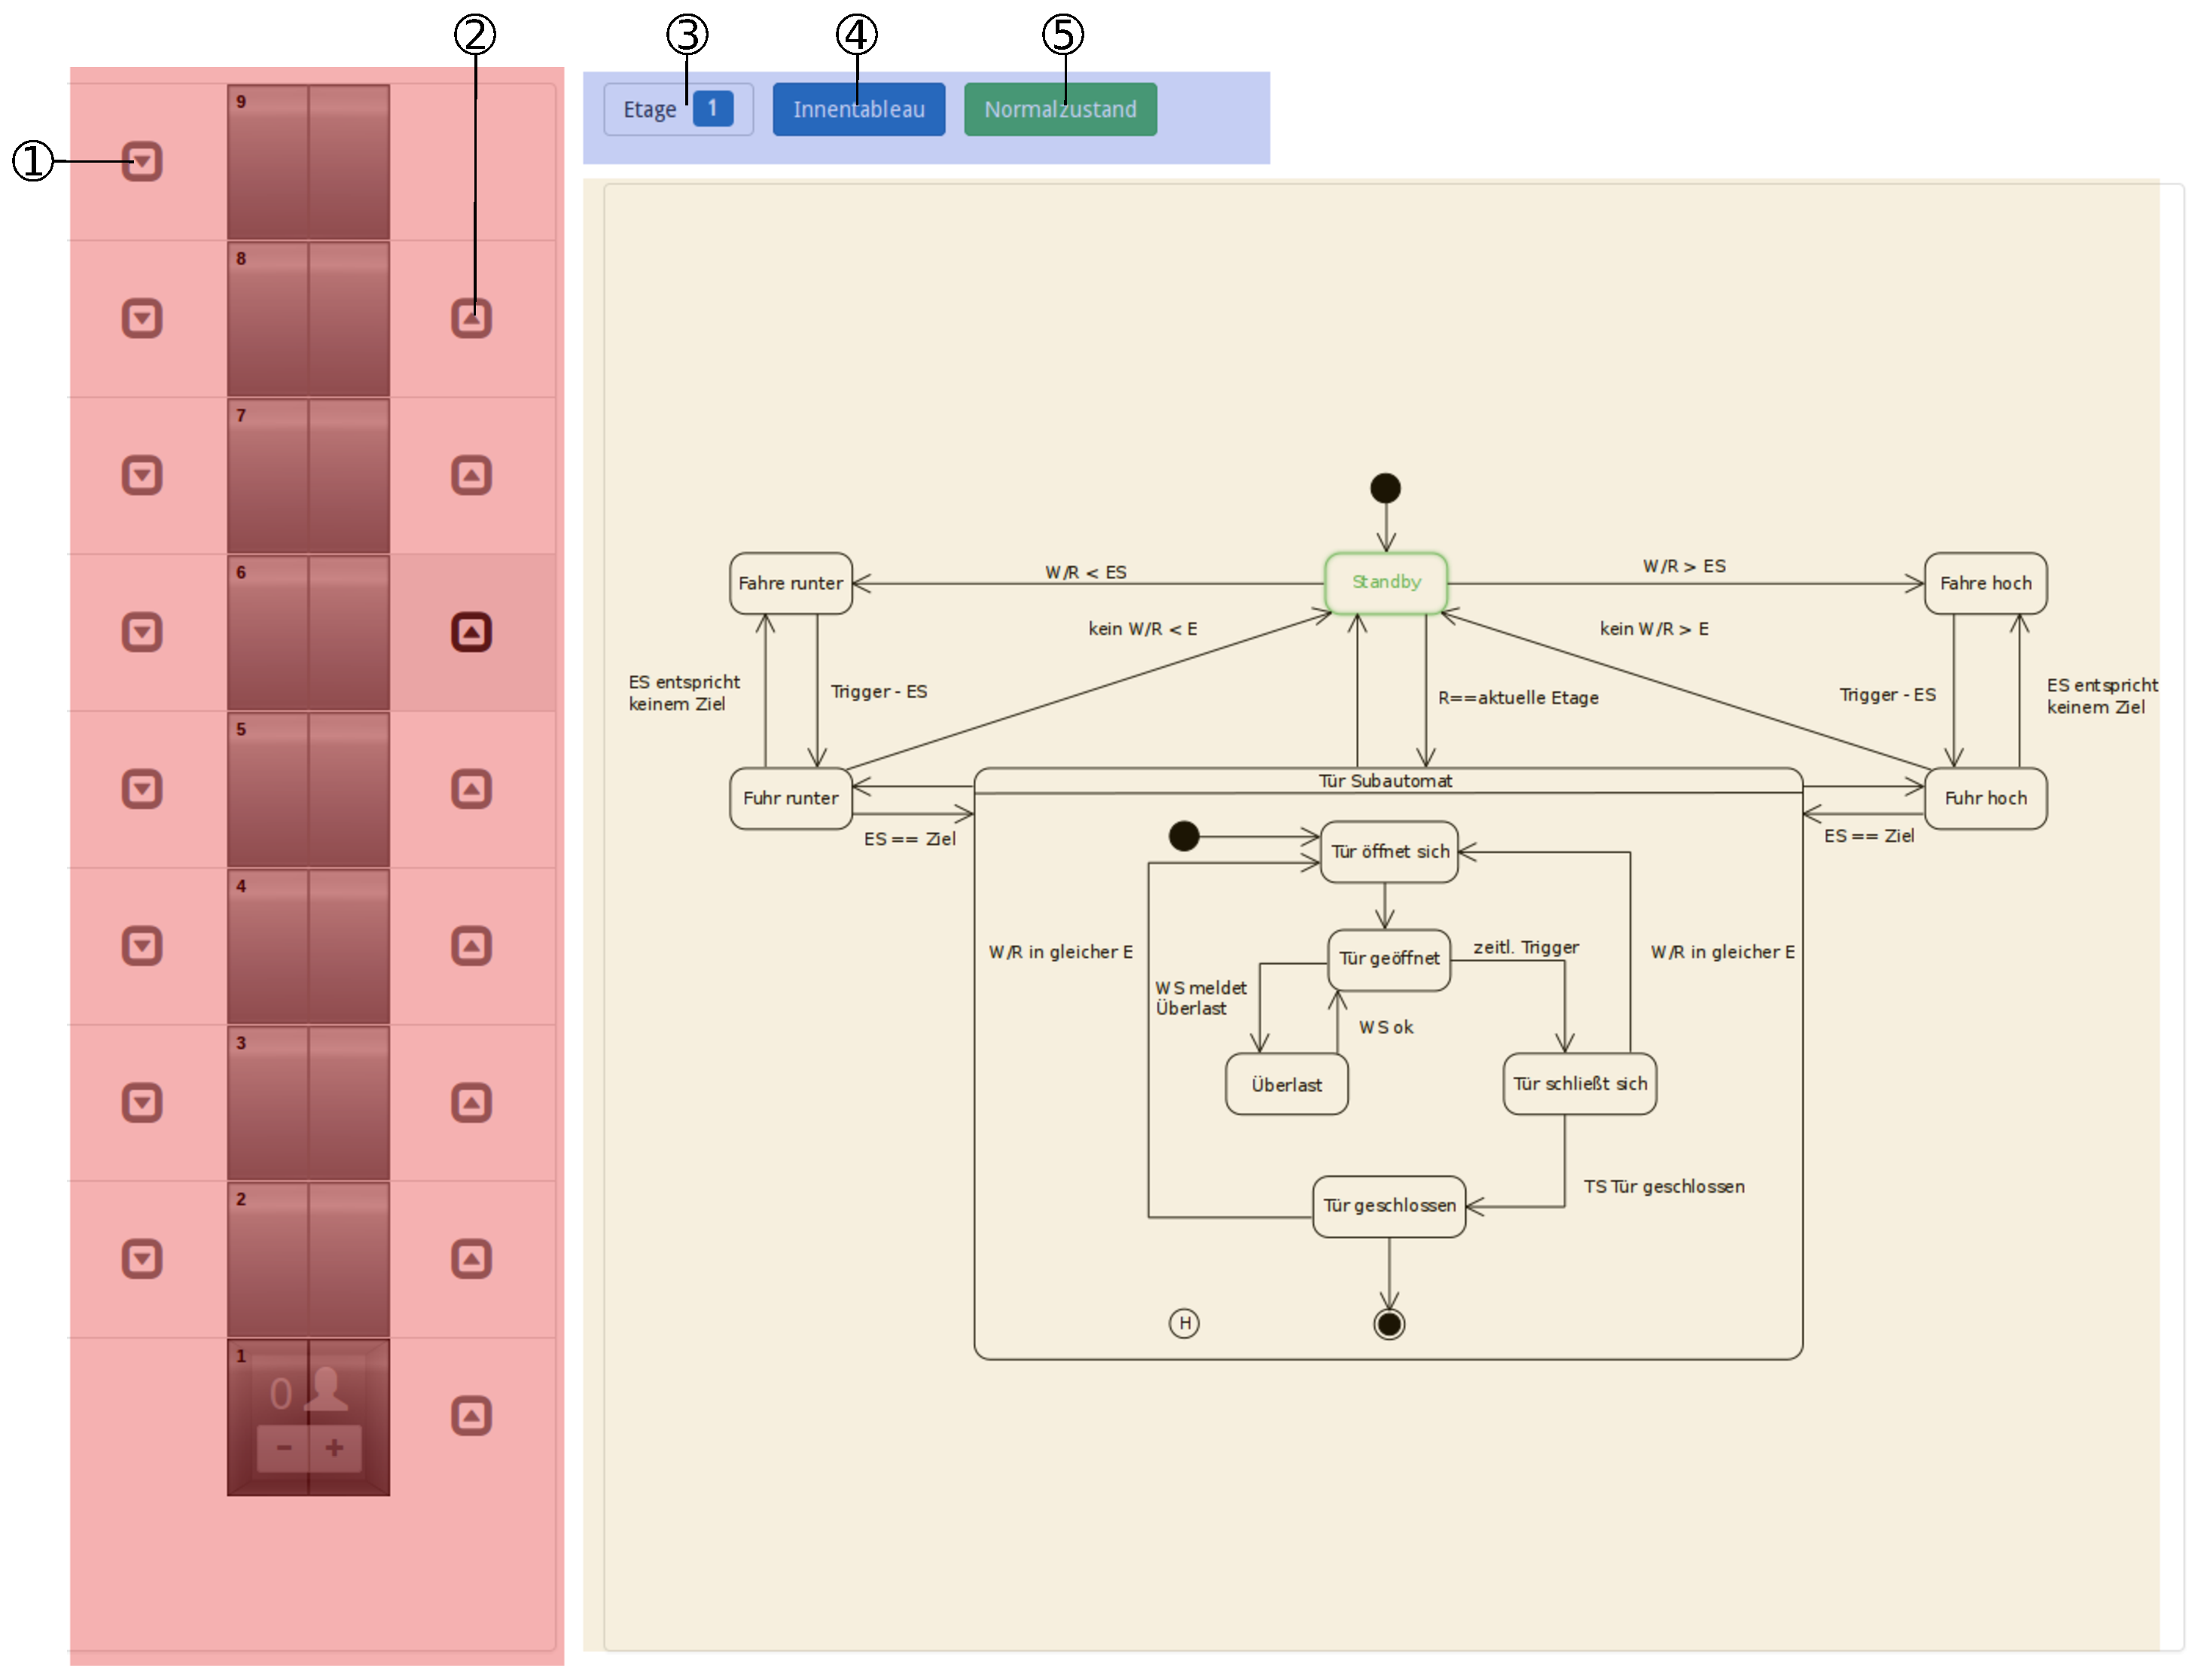
\includegraphics[width=1.2\textwidth]{images/UI.eps}
\end{figure}

\vspace*{1.5cm}
\begin{figure}[h!]
	\begin{minipage}{0.4\textwidth}
		\centering
		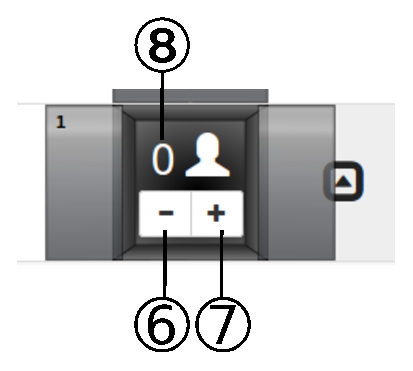
\includegraphics[width=0.9\textwidth]{images/UI_Tuer.eps}
		%\caption{Ansicht Fahrstuhlkabine}
		%\label{fig:ui_tuer}
	\end{minipage}
	% Auffüllen des Zwischenraums
	\hfill
	% minipage mit Grafik
	\begin{minipage}{0.6\textwidth}
		\vspace*{0.5cm}
		\hspace*{0.5cm}
		\begin{tabularx}{0.92\textwidth}{lX}
			1 & Fahrtruf nach unten\\ \hline
			2 & Fahrtruf nach oben\\ \hline
			3 & Anzeige der aktuellen Etage\\ \hline
			4 & Innentableau anzeigen (Maus über Button bewegen)\\ \hline
			5 & Überlastanzeige verändert\newline Farbe und Bezeichnung, bei\newline Überlastsituation\\ \hline
			6 & Passagiere einsteigen lassen\\ \hline
			7 & Passagiere aussteigen lassen\\ \hline
			8 & Anzeige der Passagiere im Fahrstuhl\\ \hline
			\label{ui_table}
		\end{tabularx}
	\end{minipage}
	\caption{Übersicht der Benutzeroberfläche}
	\label{fig:ui}
\end{figure}

\paragraph{}Durch Interaktion mit dem Fahrstuhlsystem ausgelöste Vorgänge und Zustandsübergänge werden im Hauptbereich \testclr{gelb} durch farbliche Veränderungen ansprechend dargestellt. Dabei werden folgende Farbhervorhebungen verwendet:

\begin{itemize}
	\item \testclr{state-active} Aktueller Zustand
	\item \testclr{state-last} Letzter Zustand
	\item \testclr{state-lastlast} Vorletzter Zustand
\end{itemize}

Das Anzeigen der letzten bzw. vorletzten Zustande ist erforderlich, weil einige Zustände nur sehr kurz aktiv sind und ohne entsprechende Hervorhebung nicht sichtbar wären.